\chapter{State of the Art in Retrieval-Augmented Generation}
\label{chap:sota}
\begin{spacing}{1.5}
\sloppy
In the landscape of AI, large language models (LLMs) have demonstrated remarkable results in text generation and understanding. Yet, when applied to real-world tasks such as question answering, these models still face significant limitations. As discussed in \autoref{chap:QAS}, LLMs are prone to hallucinations, rely on static and often outdated training data, and offer limited transparency or traceability in their outputs. Additionally, they may struggle to incorporate domain-specific context or organisational knowledge \parencite{vaibhav_retrieval-augmented_2025}, posing challenges for domains like cultural heritage, GLAM (Galleries, Libraries, Archives and Museums) and archaeology, where reliability, provenance, and interpretive consistency are fundamental requirements \citep{di_marcantonio_intelligenza_2024}.

To address these concerns, retrieval-augmented generation (RAG)\footnote{The terminology ``retrieval-augmented generation'' was introduced by \citeauthor{lewis_retrieval-augmented_2020} (\citeyear{lewis_retrieval-augmented_2020}) in their influential paper \textit{Retrieval-Augmented Generation for Knowledge-Intensive NLP Tasks}. Since then, the term has come to designate a broad family of methods and design patterns that combine retrieval with generative techniques, unifying diverse approaches to knowledge-grounded text generation.\\ For more information about RAG technique, see \url{https://en.wikipedia.org/wiki/Retrieval-augmented_generation}.} has emerged as a crucial methodological advance. It improves the factual grounding and contextual relevance of generated answers, through the integration of external and verifiable knowledge at inference time, thereby reducing the risk of generating fabricated or distorted information \citep{martineau_what_2023}. This approach marks a clear progression beyond both traditional IR techniques and earlier neural QA models, which were often brittle, domain-dependent, or struggled to adapt to evolving information needs.

Although initially conceived for open-domain question answering and enterprise search \parencite{akkiraju_facts_2024, jiang_towards_2024, packowski_optimizing_2024, yang_ragva_2025, zhou_enabling_2025}, RAG pipelines are are now finding growing resonance in the humanities and cultural heritage domains. In these settings, where interpretive rigour, provenance, and reliability of information are critical, they serve as valuable instruments to support scholars and professionals in navigating vast, fragmented knowledge repositories. Recent initiatives have begun to experiment with RAG for the analysis of sensitive historical materials \citep{callaghan_prototyping_2025, ciletti_retrieval-augmented_2025, sergeev_talking_2025, fan_research_2025}, underscoring its potential to support critical scholarly practices. However, the present work explores a distinct application: improving access to procedural and technical documentation, where clarity, consistency, and actionable guidance are the primary objectives.
\\

This chapter provides a comprehensive account of the state of the art in retrieval-augmented generation, situating it within the broader research landscape, clarifying its core mechanisms, and tracing its emerging applications in the digital humanities.

\section{Foundations of the Technique}\setlength{\parskip}
{0pt}
Retrieval-augmented generation (RAG) has emerged as a hybrid paradigm that tackles some of the most persistent shortcomings of LLMs, such as knowledge staleness, narrow scope of their context windows, and difficulty of tracing outputs back to their sources \citep{vaibhav_retrieval-augmented_2025,gao_retrieval-augmented_2024, gupta_comprehensive_2024}. Although LLMs excel at producing fluent, human-like text, they often falter when facing specialised queries or requests for information that falls beyond their training cutoff. RAG directly addresses these challenges by integrating external information retrieval within the generation process, allowing outputs to be more factual, up-to-date, and grounded in verifiable sources \citep{wang_searching_2024}.

At its core, a typical RAG pipeline consists of two main stages: \textbf{retrieval} and \textbf{generation} (\cite{odsc-community_retrieval-augmented_2024}). The process begins with preprocessing and indexing, where raw data is cleaned, extracted, segmented into manageable ``chunks'', and encoded into vector representations. These embeddings are then stored in a dedicated database to facilitate efficient similarity searches. When a user submits a query, it is encoded in the same vector space, and the system retrieves the top-$k$ most relevant chunks from the indexed knowledge base. In the subsequent stage, these retrieved documents are passed as context to a generative language model\footnote{In the domain of LLMs, \textit{context} carries a dual meaning. On one hand, it denotes the context window, i.e. the maximum sequence length of tokens that the model can process at once, which determines how much information can be considered simultaneously. On the other hand, it refers to the context prompt, i.e. the specific contextual material provided to the model at inference time, including retrieved evidence, instructions, and user queries. Both are critical in RAG pipelines, since the size of the context window constrains how many retrieved chunks can be incorporated, while the design of the context prompt influences how effectively the model grounds its outputs in external knowledge.} -- often based on Transformer architectures \citep{vaswani_attention_2017} -- which synthesises a response that blends the original query with external evidence, producing answers that are both coherent and contextually appropriate \citep{arslan_survey_2024}.

This modular design (\autoref{fig:rag}) enables the continuous incorporation of domain-specific and current information, overcoming the constraints of static model parameters. Recent contributions have helped to formally systematise the RAG pipeline, with frameworks delineating specific interdependent modules such as query classification, retrieval, reranking, and generation \parencite{wang_searching_2024,gao_retrieval-augmented_2024}.

\begin{figure}[H]
  \centering
  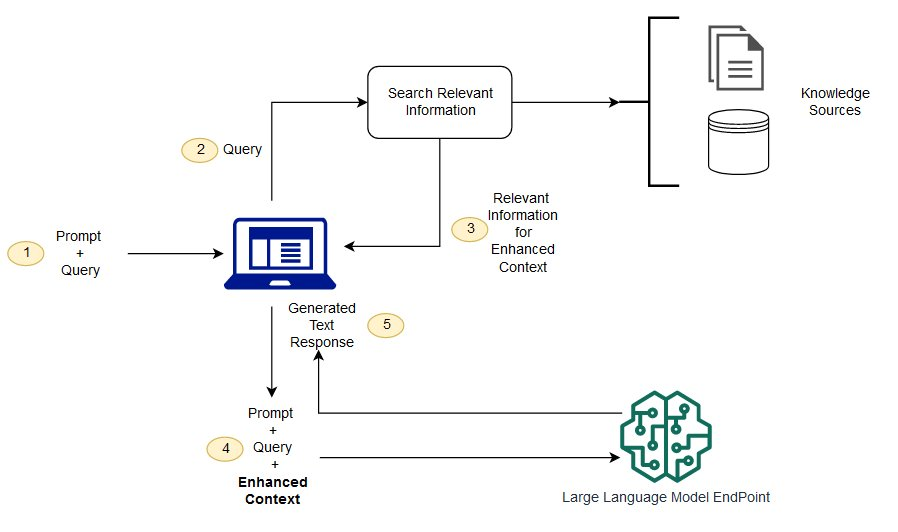
\includegraphics[width=\textwidth]{images/rag_workflow.jpg} 
  \caption{Retrieval-augmented generation pipeline combining user queries with external knowledge to produce context-aware responses.\\
  \footnotesize{Source: \url{https://aws.amazon.com/de/what-is/retrieval-augmented-generation/}.\nocite{noauthor_was_nodate}}}
  \label{fig:rag}
\end{figure}

\subsection{Pipeline Components and Common Practices}
The design of RAG pipelines can vary considerably depending on the specific use case, domain of application, and resources available. Still, a number of recurring practices have gradually crystallised into what can be regarded as the current state of the art in retrieval-augmented generation \citep{vaibhav_retrieval-augmented_2025,wang_searching_2024,arslan_survey_2024,gao_retrieval-augmented_2024,gupta_comprehensive_2024}. These practices often serve as reference blueprints rather than rigid prescriptions, since not every component needs to be implemented in every system. Instead, they represent a modular design space, where specific strategies can be combined, adapted or omitted to suit particular tasks.

In its most typical configuration, a RAG pipeline comprises the following modules:
\begin{itemize}
  \item \textbf{Query understanding and classification.} Not all queries require retrieval from external sources. Advanced systems first analyse and classify incoming queries to determine whether retrieval is necessary or if the language model alone suffices. This step relies on natural language understanding (NLU) techniques to extract key entities, relationships, and user intent, thereby improving efficiency and reducing unnecessary retrieval latency.
    \item \textbf{Document indexing and chunking.} Raw data from source documents is preprocessed, cleaned, segmented into smaller chunks at token, sentence, or semantic level, and converted into dense vector representations called embeddings. Recent studies recommend dynamic or semantic chunking over simple fixed-size splitting, as it better preserves context and improves retrieval quality -- especially in heterogeneous domains \citep{gao_precise_2022}.
    \item \textbf{Embedding and Vector Database.} Both document chunks and user queries are embedded into a shared vector space using models fine-tuned for semantic similarity -- e.g., BAAI/bge, LLM-Embedder, intfloat/e5. These vectors are stored in vector databases -- e.g., Milvus, Faiss, Qdrant --,\footnote{Vector databases such as Milvus and Qdrant extend similarity search with native metadata management and distributed scalability. Milvus, built for large-scale applications, focuses on cloud-native deployment and support for multiple indexing strategies, making it suitable for enterprise environments \parencite{2021milvus,2022manu}. Qdrant, written in Rust, is designed for high-performance real-time search and offers particularly strong metadata filtering capabilities \citep{qdrant_github_nodate}. Faiss (Facebook AI Similarity Search)  is a high-performance library developed by Meta AI that focuses on efficient vector indexing and similarity search without built-in metadata handling \citep{douze2024faiss}. In research contexts, these characteristics can be advantageous: Faiss offers speed, flexibility, and a wide choice of indexing methods, while metadata can be managed externally (e.g., through a separate mapping file), allowing full control over the experimental pipeline.} selected based on scalability, indexing strategy, and support for specific search capabilities.
    \item \textbf{Retrieval and query transformation.} When a user submits a query, it is first encoded into a vector representation and used to retrieve the top-$k$ relevant chunks from the indexed KB via similarity search. To make it more robust, the pipeline can adopt a hybrid approach based on dense retrieval -- embedding-based methods such as DPR or Contriever -- combined with sparse retrieval -- lexical methods such as BM25. Retrieval can be further improved through query transformation strategies, including rewriting, decomposition, or the generation of hypothetical supporting documents -- e.g., HyDE.
    \item \textbf{Reranking.} the initial candidate set can be reordered to emphasise relevance to the original query. This is frequently achieved with cross-encoder models -- such as monoT5, monoBERT, or RankLLaMA --, which jointly consider the query and each candidate, or with more sophisticated algorithms through heuristics. This contextualization ensures that the most pertinent information is prioritised for the generative model.\\See \autoref{tab:rerank_algorithms} for a summary on reranking techniques.
    \item \textbf{Repacking and summarization.} In some cases, retrieved passages may be reorganised or summarised to distil key information, especially when dealing with lengthy corpora. This step can involve extractive summarization or abstractive -- e.g., with Pegasus -- techniques to condense information and fit within the context window of the generator model.
    \item \textbf{Generation.} The generative model -- usually a transformer-based LLM such as T5, BART, or GPT -- synthesises a response conditioned on both the original query and the retrieved context, integrating intrinsic model knowledge with external evidence to produce a coherent, accurate, and contextually grounded answer.
\end{itemize}


\autoref{tab:best_rag} presents an overview of the methods most consistently reported as high-performing for each module of a RAG pipeline. When aiming for balanced efficiency -- i.e., reducing latency while maintaining good, but not maximal, accuracy -- adjustments are typically made at the retrieval and reranking stages. In practice, this involves replacing the Hybrid + HyDE retrieval method with a standard Hybrid search approach, which combines BM25 and dense retrieval without pseudo-document generation, and substituting monoT5 with TILDEv2 for reranking, which delivers faster processing at the cost of a modest reduction in answer quality \citep{wang_searching_2024}.

\addtocounter{table}{-1}
\begin{table}[H]
\centering
\footnotesize
\begin{tabularx}{\textwidth}{l X}
\toprule
\textbf{Algorithm} & \textbf{Rationale} \\
\midrule
Cross-encoder rerankers & Jointly encode concatenated query-document pairs to produce fine-grained relevance scores. These models -- e.g., monoT5, monoBERT, RankLLaMA -- are fine-tuned to classify relevance as ``true'' or ``false'', and at inference, documents are ranked by the predicted probability of the ``true'' label \citep{wang_searching_2024}. \\
\cmidrule(lr){1-2}
TILDE \citep{zhuang_tilde_2021} & Token-level likelihoods for queries across a collection, allowing fast reranking by summing the probabilities of query tokens given each candidate passage. \\
\cmidrule(lr){1-2}
Learning-to-Rank (LTR) \citep{gupta_comprehensive_2024} & Traditional machine learning ranking approaches: \textbf{a) Point wise:} predicts relevance score for each document independently; \textbf{b) Pair wise:} compares pairs of documents to learn relative relevance; \textbf{c) List wise:} considers the entire ranked list at once.\\
\cmidrule(lr){1-2}
HyDe \citep{gao_precise_2022}  & Generates hypothetical documents from queries for dense retrieval.\\
\cmidrule(lr){1-2}
Hybrid Search (sparse + dense scoring) & Blends scores from dense retrievers (semantic similarity -- e.g., DPR, Contriever) and sparse methods (lexical overlap -- e.g., BM25, TF-IDF) for robust ranking. Sometimes uses learnable weighting \citep{wang_searching_2024}. \\
\cmidrule(lr){1-2}
HyDE + Hybrid Search \citep{wang_searching_2024} & Combines HyDE's hypothetical document generation with hybrid search for retrieval. \\
\cmidrule(lr){1-2}
Graph-based \citep{han_retrieval-augmented_2025} & Constructs a graph of candidates (nodes) based on relationships (semantic, citation, or knowledge graph edges), then uses graph algorithms  (e.g., PageRank, label propagation) to identify central passages. \\
\cmidrule(lr){1-2}
Self-RAG (LLM-enhanced reranking) \citep{asai_self-rag_2023} & Uses LLMs directly to score or select the most relevant passages, sometimes via few-shot prompting or chain-of-thought reasoning. \\
\bottomrule
\end{tabularx}
\vspace{0.5em}
\caption{Algorithms for document retrieval and reranking in RAG pipelines}.
\label{tab:rerank_algorithms}
\end{table}



\addtocounter{table}{-1}
\begin{table}[H]
\centering
\begin{tabularx}{\textwidth}{l>{\raggedright\arraybackslash}X>{\raggedright\arraybackslash}X}
\toprule
\textbf{Module}         & \textbf{Method(s)} & \textbf{Functionality} \\
\midrule
Retrieval         & Hybrid with HyDE            & Combines Hybrid Search (BM25 + dense) and HyDE pseudo-documents. \\
\cmidrule(lr){1-3}
Reranking         & DLM w/ monoT5                      & Deep LLM-based reranker (good balance of quality and speed). \\
\cmidrule(lr){1-3}
Chunking          & Small2big / Sliding Windows & Organising chunk block relationships for context preservation. \\
\cmidrule(lr){1-3}
Embedding         & LLM-Embedder                & Dense supervised retriever, best trade-off performance/size. \\
\cmidrule(lr){1-3}
Vector Database   & Milvus                      & Best coverage of index type, scalability, hybrid search, cloud-native. \\
\cmidrule(lr){1-3}
Repacking         & Reverse                     & Puts most relevant context close to the query. \\
\cmidrule(lr){1-3}
Summarization     & Recomp                      & Both extractive and abstractive methods tested; Recomp performs best. \\
\bottomrule
\end{tabularx}
\vspace{0.5em}
\caption{Best-performing RAG pipeline configurations across modules, selected for maximising performance w.r.t. answer quality and accuracy.}
\label{tab:best_rag}
\end{table}

\autoref{fig:summary_rag} provides a broader overview of the RAG ecosystem. The paradigm evolves from naive to modular RAG, incorporating techniques for improving retrieval and generation -- e.g., chunk optimization, adaptive retrieval, dual fine-tuning --, as well as the key issues of when, what, and how to retrieve. RAG also faces open challenges, including robustness, scaling laws, production readiness, alongside modality extensions to image, audio, video, code, and ecosystem directions like customization, specialization. Finally, current evaluation targets and frameworks distinguish between retrieval quality and generation quality, together with their assessment aspects such as answer relevance, context relevance, faithfulness, robustness, and integration \citep{gao_retrieval-augmented_2024}.

\begin{figure}[H]
  \centering
  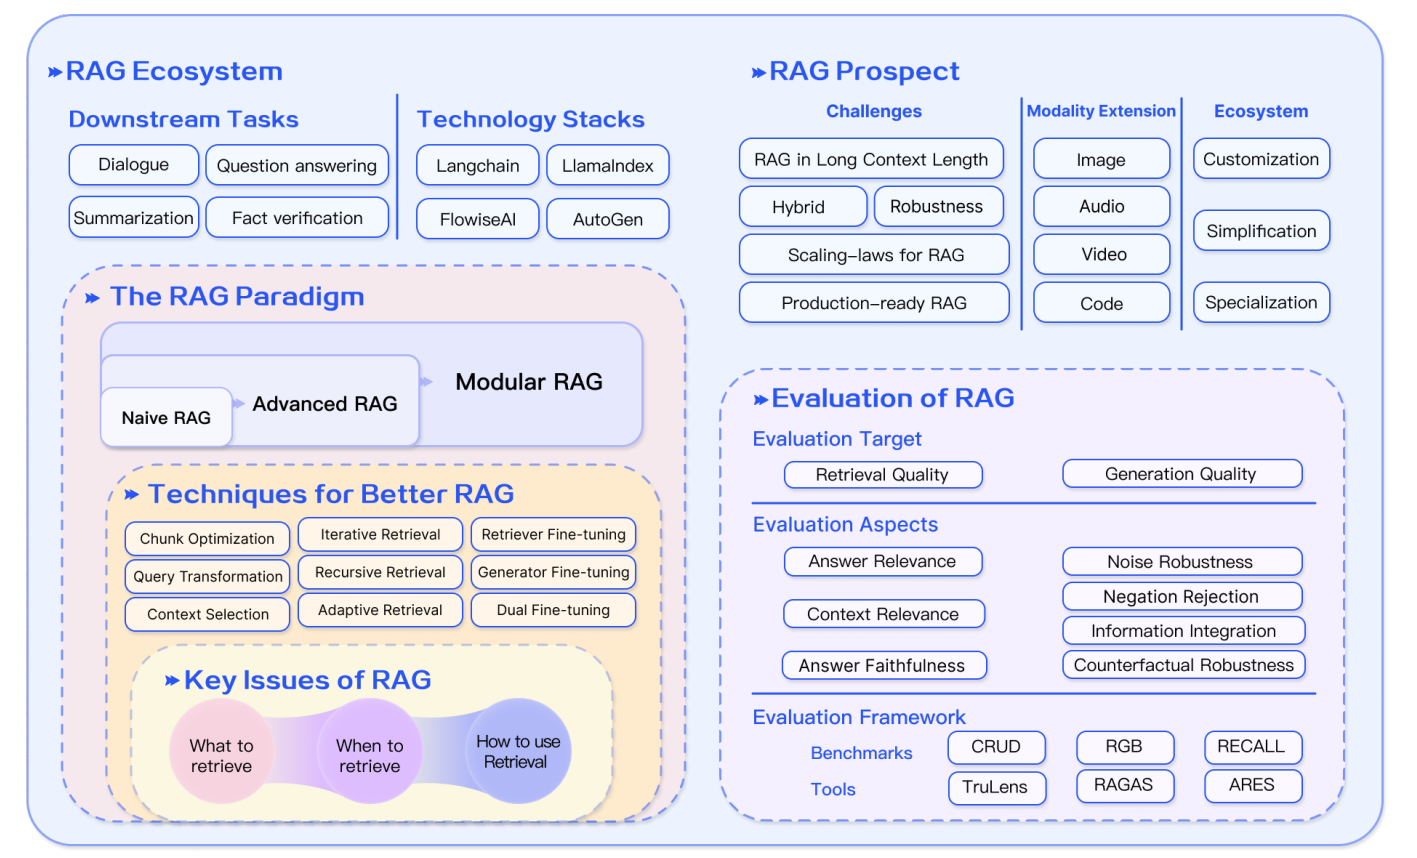
\includegraphics[width=\textwidth]{images/RAG_ecosystem.png} 
  \caption{Summary overview of the RAG ecosystem.\\
  \footnotesize{Source: \cite{gao_retrieval-augmented_2024}}.}
  \label{fig:summary_rag}
\end{figure}

\subsection{Evaluation and Benchmarking}\label{sec:eval_and_bench}
Evaluating RAG systems poses unique challenges, as traditional metrics like BLEU, ROUGE or METEOR may not fully capture the quality of generated responses, particularly in terms of factual accuracy and contextual relevance \citep{deriu_survey_2020}. In conversational QA research, this limitation has long been acknowledged, as multi-turn settings require models to answer a single query and to maintain consistency, resolve co-references, and adapt to evolving conversational context \citep{zaib_conversational_2022}. Consequently, evaluation must go beyond surface level overlap and incorporate measures that reflect contextual appropriateness and understanding at discourse level. Moreover, assessing RAG systems requires attention to both retrieval and generation quality, since failures in either stage directly impact the final response \citep{abeysinghe_challenges_2024}.

Surveys of the field increasingly stress the need for frameworks capable of measuring multiple dimensions of RAG. Despite the rapid advancements in retrieval, generation, and augmentation, evaluation methods remain underdeveloped, with persistent challenges in capturing retrieval quality, hallucination rates, and faithfulness of generated content in a systematic way \citep{gao_retrieval-augmented_2024}. Large-scale benchmarks such as TREC \citep{voorhees_trec_2005}, MS MARCO \citep{bajaj_ms_2018} and BEIR \citep{thakur_beir_2021} continue to be standard for retrieval, but generation quality requires different approaches. Newer frameworks like the \textit{Retrieval-Augmented Generation Assessment System (RAGAS)} have therefore been introduced to capture aspects such as contextual alignment, answer faithfulness, and pipeline-level performance \citep{es_ragas_2023}.

Experimental studies of RAG pipelines within LLM-based applications further demonstrate the complexity of the task. For example, a recent work compares automated metrics, human evaluation, and LLM-based evaluation in the context of \textit{EdTalk}, a RAG-powered chatbot built to navigate educational reports. Their findings show that automated metrics such as BLEURT are useful for rapid iteration but often misalign with human judgments, while factored human evaluation -- structured around criteria including correctness, informativeness, relevance, clarity, and hallucination -- provides richer insights into system performance. At the same time, LLM-based evaluators show promise for scalable assessment but risk inflating scores, especially when the same model is used for both generation and evaluation. This stresses the need for hybrid and carefully designed evaluation pipelines when deploying RAG in real-world contexts \citep{abeysinghe_challenges_2024}.

Human-in-the-loop assessment remains indispensable, with expert judges assessing criteria such as factual accuracy, coherence, and domain relevance -- offering richer and often more reliable quality assessments than quantitative metrics alone. In conversational contexts, this is especially important, as metrics must reflect user satisfaction and interaction quality rather than isolated response correctness \citep{gupta_comprehensive_2024}.

Alongside automated and human-centred metrics, evaluation taxonomies are moving toward a more fine-grained view of system quality. Dimensions such as answer relevance, context relevance, and faithfulness directly address hallucination and grounding, while robustness dimensions -- including resilience to noise, negation, counterfactual scenarios, and multi-source information integration -- test whether systems remain reliable under real-world conditions. To operationalise these dimensions, new benchmarks such as CRUD, RGB, and RECALL extend beyond traditional IR settings by jointly assessing retrieval and generation. Complementary tools make evaluation continuous and developer-friendly: RAGAS targets faithfulness and contextual alignment, ARES offers flexible automated pipelines, and TruLens integrates performance monitoring into deployed workflows \citep{gao_retrieval-augmented_2024}.

Furthermore, ethical considerations must be embedded throughout the lifecycle of RAG pipelines. Protecting data privacy, mitigating algorithmic bias, and complying with regulations such as GDPR are fundamental. This means adopting technical measures like privacy by design, data minimisation, and access control, in addition to committing to broader ethical principles widely recognised in international guidelines: transparency, justice and fairness, non-maleficence and responsibility \citep{jobin_global_2019}. Ongoing audits, stakeholder involvement, and mechanisms for accountability, including whistleblowing and legal clarity, help bridge the gap between abstract principles and operational practice, ensuring systems remain trustworthy and socially beneficial \citep{ashery_emergent_2025}.

Overall, the line of evolution of RAG systems points toward increasingly sophisticated applications that are deeply integrated into the workflows of research, industry, and cultural institutions. Innovations in evaluation frameworks, user interaction, and system scalability are steadily pushing the boundaries of what these models can achieve. As these technologies continue to mature, success will depend on the ability to combine robust benchmarking, user-centred feedback mechanisms, and adaptive optimisation strategies. Overcoming challenges related to factuality, scalability, and responsible deployment will be essential for building trustworthy systems capable of delivering high-quality information in context-sensitive settings. Looking ahead, continued advances in RAG are set to play a pivotal role in shaping the future of digital knowledge access and discovery, and establish it as a cornerstone technology \citep{zaib_conversational_2022,wang_searching_2024, gao_retrieval-augmented_2024}.

\section{New Frontiers Applications}\label{sec:evol_qas}
RAG systems are increasingly deployed across a wide spectrum of contexts -- spanning academic research, enterprise infrastructures, and real-world product environments -- where they serve to enhance data accessibility, support decision-making, and facilitate natural language interaction with complex KBs. Recent surveys and empirical studies trace a rapidly expanding set of scholarly applications. In the context of academic support, for instance, retrieval-augmented pipelines power automated literature review tools and citation management platforms such as \textit{LitLLM} \citep{agarwal_litllm_2025}, and \textit{KNIMEZoBot} \citep{alshammari_knimezobot_2023}. In conversational AI, advanced retrieval enables grounded multi-turn dialogue, exemplified by \textit{Wizard of Wikipedia (WoW)} \citep{dinan_wizard_2019}, which can be read as an early instantiation of what is now formalised as RAG-based dialogue modelling. The paradigm is also leveraged for large-scale summarisation, distilling insights across vast corpora of scholarly papers, and for fact verification tasks, as in resources like \textit{PubHealth}, increasingly adopted to counter misinformation in sensitive domains such as health communication \citep{kotonya_explainable_2020}. In this regard, RAG has proven especially valuable in domain-specific knowledge extraction, most notably in biomedical and legal research, where retrieval mechanisms act as an extension of expert knowledge.


In one experiment, a RAG system was developed to assist data scientists through a combination of GROBID library\footnote{GROBID is a machine learning library designed to extract, parse, and convert raw documents, like PDFs, structured XML/TEI encoded documents \citep{GROBID}.} for structured bibliographic extraction, fine-tuned embeddings, semantic chunking, and an abstract-first retrieval strategy. The system's performance, assessed using RAGAS, demonstrated improved faithfulness and context relevance in response generation \citep{aytar_retrieval-augmented_2024}. A similar approach was explored in the context of academic library systems, where RAG was applied to improve contextual retrieval through semantic indexing of structured metadata -- e.g., MARC/RDA standards -- and multimodal resources. Additionally, the framework introduced conversational querying via a natural language interface, supporting compound interdisciplinary searches and significantly improving document discoverability by synthesising citation-backed responses from diverse scholarly sources -- including journals, datasets, and videos; this solution also addressed challenges such as copyright compliance and ethical AI transparency \citep{bevara_prospects_2025}.  Collectively, these studies affirm the efficacy of RAG systems in alleviating information overload and improving research workflow discoverability.

In parallel, further critical insights into the design of RAG systems for domain-specific and technical content have been highlighted in recent work \citep{soman_observations_2024}, which closely aligns with the methodological framework adopted in the GNA question-answering system. Using IEEE telecommunications engineering corpora -- i.e., wireless LAN specifications and battery glossaries -- as testbeds, their analysis highlights key factors influencing retrieval quality, which include chunk size, sentence-level similarity, and the strategic placement of domain-specific terms. These aspects are similarly addressed in the GNA RAG pipeline \citep{pograri_question-answering_2025}, which applies customised chunking, semantic preprocessing, and contextual embedding strategies. Both studies advocate for more nuanced and contextually informed approaches to enhance precision in technical and highly structured domains.

Numerous recent graduate-level research projects have provided substantive input into the implementation and evaluation of RAG systems:
\begin{itemize}
    \item \textcite{antolini_experimental_2025} developed a custom RAG system for open-domain question answering using both traditional (BM25, PRF) and advanced retrieval strategies, integrated with local LLMs. A novel Parametric RAG (PRAG) approach was also explored, embedding context into model parameters for performance gains;
    \item \textcite{caramanna_progettazione_2024} investigated conversational agent architectures, comparing various LLM types and retrieval configurations;
    \item \textcite{florio_progettazione_2024} implemented a LangChain-based RAG chatbot for corporate documentation, evaluating multiple vector database technologies.
    \item \textcite{salcuni_utilizzo_2025} applied RAG to the medical domain, improving LLM responses in hypertension care. The study used RAGAS to assess quality and relevance, focusing on personalization and accuracy;
    \item \textcite{nicoletti_llms_2025} developed Essence Coach, a chatbot that integrates LLMs with the Essence software engineering standard. This system significantly outperformed generic LLMs like GPT-4o in domain-specific reasoning tasks.
\end{itemize}

\section{Retrieval-Augmented Generation in the Digital Humanities}\label{sec:rag_dh}
A growing body of research is exploring RAG applications within the digital humanities. One such example is the \textit{iREAL} project, which applied RAG to interpret archival records from Aboriginal schools in Australia, demonstrating a careful balance between cultural sensitivity and historical accuracy \citep{callaghan_prototyping_2025}. Another initiative, \textit{ValuesRAG}, focuses on cultural alignment in LLMs by integrating societal and demographic knowledge through retrieval-augmented contextual learning, experimenting with the \textit{World Values Survey} dataset \citep{seo_valuesrag_2025}. In another case, the \textit{Foggia Occupator Dataset} project applied a RAG model to post-WWII Italian periodicals, extracting information on political figures and stylistic traits \citep{ciletti_retrieval-augmented_2025}.

Among the technical approaches explored in recent experiments on generative AI for digital scholarly editions (DSEs), RAG emerges as a promising method for addressing challenges such as entity linking (EL) and the integration of external knowledge sources. Notably, RAG is recognised for its ability to mitigate hallucinations in named entity recognition (NER) and to enable the enrichment of text with information from structured databases or knowledge graphs \citep{pollin_when_2025}. For example, an experiment with the \href{https://www.regesta-imperii.de/en/home.html}{Regesta Imperii project}\nocite{noauthor_home_nodate} demonstrates how knowledge bases, including Neo4j graph databases, are leveraged within RAG pipelines to improve accuracy in information extraction, entity normalization, and semantic annotation \citep{kuczera_chatgpt_2024}. Similarly, the editorial workflow developed for the \href{https://web.archive.org/web/20241120122545/https://gams.uni-graz.at/context:hsa}{Hugo Schuchardt Archive} outlines a process that combines prompt engineering, human-in-the-loop oversight, and RAG tool chains to enhance the generation of TEI-compliant XML, supporting more explainable and modular processing pipelines \citep{pollin_new_2023}. These and other experiments underscore the need for standardised workflows, robust evaluation protocols, and systematic research into both the strengths and weaknesses of LLMs and related tools in the editorial process, while also advocating for thoughtful engagement with advanced computational methods in the humanities \citep{pollin_workshop_2024}. As digital editions become increasingly complex and interconnected with broader knowledge infrastructures, the relevance and application of AI technologies such as RAG are both expected and desirable to grow accordingly.

RAG methodologies are being adopted within the GLAM sector as well. In archival contexts, a smart assistant developed for querying the \textit{Prozhito} digital archive of personal diaries combines text-to-SQL filtering, hybrid search, and automatic query reformulation, proving especially effective for historians and anthropologists without prior knowledge of database query languages  \citep{sergeev_talking_2025}. Meanwhile, in museum settings, a comparative evaluation of RAG techniques versus direct large-context input approaches -- i.e., feeding the entire context at once to a language model -- for answering multimodal questions about artworks demonstrated that large-context models generally give more accurate answers than RAG, at least for this task and dataset. However, RAG remains useful when information exceeds context window limits or when efficiency is important \citep{ramos-varela_context_2025}.

Innovations in graph-based retrieval are also gaining momentum. Techniques combining structured supervision and chain-of-thought prompting have been used to map character relationships in early modern English historiography, thereby reducing the manual workload typically associated with historical data annotation \citep{fan_research_2025}. Related directions are being explored within cultural heritage institutions, as seen in the \textit{CAT-IA} initiative, which integrates ArCo knowledge graph \citep{carriero_arco_2019} within a RAG system for provenance tracking, AI explainability (XAI), and structured metadata extraction \citep{barbato_nasce_2025}. Designed to streamline and enrich user interactions with the General Catalogue of Cultural Heritage \textit{(Catalogo generale dei beni culturali)}, \textit{CAT-IA} marks a notable stride in applying advanced digital technologies to promote accessibility and valorization of cultural assets.

A complementary, conceptual perspective emerges in a critical mapping of the theoretical contours of RAG within the broader landscape of archives, libraries, and cultural heritage, articulating the potential for RAG-augmented LLMs to enhance the precision, accessibility, and contextualization of information retrieval, and foregrounding the social and infrastructural challenges inherent in such integration. This viewpoint encourages the field to reflect on both the affordances and the epistemic and ethical complexities introduced by RAG systems in digital humanities contexts \citep{di_marcantonio_intelligenza_2024}.


Finally, efforts to advance access to fragmented digital repositories -- such as web archives -- have increasingly adopted RAG methodologies. An illustrative bespoke prototype transforms keyword-based search into semantically guided question answering \citep{davis_unlocking_2025}, sharing architectural parallels with the GNA QA system presented in the context of this thesis. Both systems prioritise semantic retrieval over lexical matching using dense embeddings -- e.g., \textit{E5} variants \citep{wang_text_2024} -- to interpret queries in context, employ structured text processing pipelines to reduce noise in source materials, and apply optimised chunking strategies for retrieval accuracy. Crucially, these studies highlight RAG’s potential to transform scattered and heterogeneous resources -- whether web archives or catalographic procedures -- into coherent, accessible knowledge through contextual synthesis.

\section{Future Directions}
Ongoing research is rapidly pushing the frontiers of RAG, opening up new avenues  that extend well beyond traditional information retrieval into domains such as scientific research and the digital humanities. Among the most promising innovations, is the use of synthetic corpora to bolster the robustness and generalizability of RAG systems, particularly in low-resource or specialised domains where annotated data is scarce \citep{bor-woei_generative_2024}. This strategy improves retrieval accuracy while addressing longstanding issues of bias, coverage, and representativity in humanities corpora. 

RAG is also at the core of a new wave of applications that automate and enhance scholarly practices. In scientific research, advanced RAG frameworks -- including agentic systems like \textit{PaperQA} \citep{lala_paperqa_2023} -- are being leveraged to conduct systematic literature reviews, automate evidence synthesis, summarise emerging trends, and provide transparent citation recommendations. Particularly, these multi-stage architectures enable recursive reasoning and dynamic tool usage, often surpassing human-level performance in both retrieval and summary tasks \citep{skarlinski_language_2024}. 

Despite these advances, several critical research challenges remain. There is an urgent need to develop domain-adapted and multilingual LLMs that can process not just text, but also multimodal data such as images, tables, and audiovisual materials -- a key requirement for both scientific and cultural heritage applications. Future RAG systems should be able to retrieve and reason over heterogeneous, cross-domain sources, necessitating robust mechanisms for evaluation, source citation, multimodal fusion, and trust calibration. The ongoing development of benchmarks and evaluation datasets, tailored to the peculiar needs of fields such as the digital humanities, is essential to guide progress and ensure methodological rigour \citep{yue_survey_2025}.

Another major direction is the semantic enrichment of RAG pipelines through the integration of ontologies and knowledge graphs. Ontologies, as formal domain knowledge models, provide structured frameworks that enable more precise and explainable retrieval semantic coherence, and the inclusion of ethical dimensions in generative AI. Complementing this, knowledge graphs capture complex relationships and support context-aware multi-hop reasoning, improving accuracy, explainability, and cultural sensitivity of outputs. Current research and practical applications in this direction span a range of initiatives, from ontology-guided entity typing to the grounding of AI in explicit ethical and procedural knowledge, demonstrating that these semantic tools are essential for creating robust and transparent RAG systems, addressing challenges in fields as diverse as healthcare, engineering, scientific discovery, and enterprise knowledge management \citep{tiwari_ontorag_2025, ludwig_ontology-based_2025, bran_ontology-retrieval_2024, sharma_og-rag_2024, xiao_orag_2024, park_ontology-based_2024, debellis_integrating_2024,franco_ontology-based_2020}.

In the specific context of the digital humanities, the accelerated adoption of AI is shaping a transformative future for scholarship, curation, and access to cultural heritage. The diverse case studies and technical innovations, discussed in \autoref{sec:rag_dh}, illustrate both the breadth of RAG’s impact and the field’s growing ambition. Across applications, from DSEs, to archival assistance and museum information systems, RAG is emerging as a pivotal enabler for addressing the limitations of traditional search and annotation by supporting contextually grounded, semantically rich, and explainable information access.

Looking forward, several converging trends and open challenges will define the evolution of RAG in the digital humanities. First, technical advances such as the integration of knowledge graphs, graph-based retrieval, and multimodal pipelines are driving improvements in semantic linking and annotation of historical, literary, and artistic materials. Second, the increasing complexity of digital scholarly editions and GLAM infrastructures is catalysing demand for standardised, reproducible workflows, robust evaluation protocols, and domain-adapted benchmarks, ensuring that RAG methods are critically assessed and tuned for the nuanced needs of humanistic research.

At the same time, as digital repositories become ever more fragmented, the promise of RAG lies in its ability to synthesise heterogeneous, dispersed data, transforming scattered web archives, periodicals, and catalogues into knowledge spaces that are accessible and meaningfully structured. Yet, this evolution also foregrounds critical conceptual and ethical questions. As highlighted by recent critical perspectives, it is essential to position RAG as an augmentative technology: one that enhances, but does not replace, established cataloguing, metadata, and interpretive practices. Human interpretive oversight, transparency, and cultural sensitivity must remain central, particularly as RAG systems are increasingly relied upon for knowledge production and mediation in complex social and historical domains \citep{di_marcantonio_intelligenza_2024}.

In sum, the next phase of RAG’s development in the digital humanities will require sustained interdisciplinary collaboration and critical reflection. Researchers and practitioners must continue to experiment with new strategies, but also engage deeply with the epistemic, social, and infrastructural complexities of integrating advanced AI into cultural knowledge management and disciplines. Ultimately, RAG applications stand poised not only to offer improved access to information, but they also invite a reimagining of the relationship between artificial intelligence and cultural knowledge production, fostering tools that augment -- not displace -- human creativity and understanding.
\end{spacing}